\documentclass{article}
\usepackage{amsmath}
\usepackage{xcolor}
\usepackage{amsthm}
\usepackage{graphicx}
\usepackage{unicode-math}
\usepackage{hyperref}
\usepackage{datetime}
\usepackage{todonotes}
\usepackage{bbm}

% inline comments
% you could use \listoftodos to print an overview
\newcommand{\inline}[1]{ {\color{blue}{#1}}\addcontentsline{tdo}{todo}{#1}}
\newcommand{\comment}[1]{{\color{blue}\noindent{#1}\\}\addcontentsline{tdo}{todo}{#1}}
% use this one to disable
%\newcommand{\inline}[1]{\ignorespaces}


\newdateformat{monthyeardate}{\monthname[\THEMONTH] \THEYEAR}

\newcommand{\newmarkedtheorem}[1]{%
  \newenvironment{#1}
    {\pushQED{\qed}\csname inner@#1\endcsname}
    {\popQED\csname endinner@#1\endcsname}%
  \newtheorem{inner@#1}%
}

\theoremstyle{definition}
%\newtheorem{eg}{Example}[section]
\newmarkedtheorem{eg}{Example}[section]
\newtheorem{observation}{Observation}[section]
\theoremstyle{plain}
\newtheorem{define}{Definition}[section]
\newtheorem{proposition}{Proposition}[section]
\newtheorem{theorem}{Theorem}[section]
\newtheorem{assump}{Assumption}[section]
\newtheorem{remark}{Remark}[section]


\title{Learning dispatching policies for the Single Intersection Scheduling problem}
\author{Jeroen van Riel}
\date{\monthyeardate\today}

\begin{document}

\maketitle

\section{Introduction}

Recall our definition of the Single Interesection Scheduling Problem. Suppose we
have a single intersection with $K$ incoming lanes. Let
$i \in \{0, \dots, K - 1\}$ be an arbitrary lane and let $n_{i}$ denote the
(possibly infinite) number of total arriving platoons to this lane. We will
refer to the $j$-th platoon of vehicles on lane $i$ as \textit{platoon}
$(i, j)$, and we let $Z_{ij} = (R_{ij}, P_{ij})$ be its full specification,
where $R_{ij}$ and $P_{ij}$ denote the release date and platoon length,
respectively. Note that we do not need to treat vehicles individually due to the
Platoon Preservation Theorem.
% arrival processes
The \textit{arrival process} of lane $i$ is defined as the collection of random variables
\begin{align}
  Z_{i} = { (Z_{ij}) }_{j=1}^{n_{i}} .
\end{align}
We saw that the Single Intersection Scheduling Problem corresponding to a
particular sample
\begin{align}
  z = {( z_{i} )}_{i=0}^{K-1} \sim Z = {( Z_{i} )}_{i=0}^{K-1} ,
\end{align}
can be concisely formulated as a Mixed-Integer Linear Program. Therefore, one
direct solution approach is to apply standard software for solving this
well-defined class of problems.

Recall that the objective of the Single Intersection Scheduling Problem was to minimize the total completion time
\begin{align}
  \sum_{i=0}^{K-1} \sum_{j=1}^{n_{i}} C_{ij}
\end{align}
over all vehicles and lanes.
%
To make comparing objective values a bit easier, we will focus on the total delay, defined as
\begin{align}
  D_{z}(y) = \sum_{i=0}^{K-1} \sum_{j=1}^{n_{i}} p_{ij} (y_{ij} - r_{ij}) .
\end{align}
for some problem instance $z$ and some feasible schedule $y$.


\section{Markov Decision Process}

% main idea: dispatching
An alternative approach is to cast the problem in terms of iteratively deciding
which platoon crosses the intersection next, to which we will refer as
\textit{dispatching}. The resulting sequential decision problem can be formulated as a
Markov Decision Process, which allows us to apply reinforcement learning
techniques.

% states
\noindent
\textbf{States.}
For each time step $t=0,1,2,\dots$, let $x^{(t)}$ denote the lane that was last
served and let $C^{(t)}$ denote the completion time of the last platoon that was
dispatched. Furthermore, let $m^{(t)}$ be a vector where entry $m_{i}^{(t)}$ counts the number of dispatched
platoons from lane $i$.
The state at step $t$ can then be written as
\begin{align}
   s^{(t)} = (x^{(t)}, C^{(t)}, m^{(t)}, z) .
\end{align}
In particular, the initial state is given by
\begin{align}
   s^{(0)} = (0, 0, 0, z ) .
\end{align}

% actions
\noindent
\textbf{Actions.}
At every state transition, some platoon is dispatched.
The action $a$ is to decide whether to keep serving the
current lane ($a = 0$), or to serve the next lane ($a = 1$).

% compute the starting times from the state
% Note that we do not consider the starting times $z_{ij}$ to be explicitly part
% of the state, because only completion time $C^{(t)}$ of the last scheduled
% platoon is necessary for the state to be Markovian.

% transitions
\noindent
\textbf{Transitions.}
The value of $x^{(t)}$ is simply updated as
\begin{align}
  x^{(t+1)} = \begin{cases}
                x^{(t)} \; & \text{ if } a^{(t)} = 0, \\
                x^{(t)} + 1 \mod K \; & \text{ if } a^{(t)} = 1.
              \end{cases}
\end{align}
The platoon that is dispatched in the transition from $t$ to $t+1$ is identified by the indices $(i^{(t)},j^{(t)})$, defined as
\begin{subequations}
\begin{align}
i^{(t)} &= x^{(t+1)} , \\
j^{(t)} &= m_{i^{(t)}}^{(t)} + 1 .
\end{align}
\end{subequations}
Therefore, the completion time $C^{(t+1)}$ of the dispatched platoon is given by
\begin{align}
  \label{eq:completion_time_update}
  C^{(t+1)} = \max\left( C^{(t)} + s a^{(t)} , \; r_{i^{(t)}j^{(t)}} \right) + p_{i^{(t)}j^{(t)}} ,
\end{align}
where $s$ is the switch-over time.
The platoon counters are simply updated as
\begin{align}
  m_{i}^{(t+1)} = m_{i}^{(t)} + \mathbb{1}\{ i = i^{(t)} \} .
\end{align}
The remaining part of the state does not change.

% reward
\noindent
\textbf{Rewards.} Recall that we assumed for the Single Intersection Scheduling Problem
that all processing times are identical $p_{j} = p = 1$. In the current MDP, we
allow platoons of arbitrary \textit{processing time}, so in order to compare
results, we assume that $p_{ij}$ is always a positive integer.
%
Observe that the delay for each vehicle in the dispatched platoon
is equal and given by
\begin{align}
  C^{(t)} - p_{i^{(t)}j^{(t)}} - r_{i^{(t)}j^{(t)}} ,
\end{align}
so the total contribution of $(i^{(t)},j^{(t)})$ to the total delay is given by
\begin{align}
  d^{(t)} = p_{i^{(t)}j^{(t)}} ( C^{(t)} - p_{i^{(t)}j^{(t)}} - r_{i^{(t)}j^{(t)}}) ,
\end{align}
which is the negative reward (cost) of step $t$. Let $N = n_{0} + \cdots + n_{K-1}$ be
the total number of platoons. Assuming $N < \infty$, the total negative reward is
precisely the total delay
\begin{align}
  D_{z}(y) = \sum_{t=1}^{N} d^{(t)}
\end{align}
for the resulting schedule $y$.

\subsection{Partial observability}

% where is the randomness?
Note that the exact arrivals $z$ are a constant part of the state and that all
transitions are deterministic. The only randomness in the MDP stems from the
distribution of the initial state, which is essentially the distribution of $Z$.
This model fits the assumption that all future arrivals are known to the
scheduler in advance. Alternatively, we could assume that the number of known
future arrivals is limited. Let us first model this in terms of
\textit{observations}, thereby obtaining a Partially Observable Markov Decision
Process (POMDP).

% observations
Assume that the scheduler does not know about all arrivals upfront, but sees
a certain number $h$ of next arrivals at every lane $i$, then the
visible \textit{horizon} of lane $i$ at step $t$ consists of the release dates
and processing times
\begin{align}
  \label{eq:observations}
  h_{i}^{(t)} = ( z_{ij} : m_{i}^{(t)} \leq j \leq m_{i}^{(t)} + h ) .
  % h_{i}^{(t)} = {( z_{i})}_{j=m_{i}^{(t)}}^{m_{i}^{(t)} + h} .
\end{align}
Therefore, the observation at step $t$ is deterministic and given by
\begin{align}
  h^{(t)} = {( h_{i}^{(t)} )}_{i=0}^{K-1} .
\end{align}

% POMDP -> MDP
Because the arrival process is independent of the actions that are taken by the
scheduler, the POMDP can simply be reformulated as a MDP\@. Instead of sampling
the full arrival process at the initial state, we can assume that some next
platoon is sampled at every transition.
In that case, the states should be written as
\begin{align}
  s^{(t)} = (x^{(t)}, C^{(t)}, m^{(t)}, z^{(t)}) .
\end{align}
%
In the initial state, we have
\begin{align}
  z_{i}^{(0)} = {( Z_{ij} )}_{j=1}^{h} ,
\end{align}
for each lane $i$.
%
For the lane $i=i^{(t)}$ that was served in the transition from step $t$,
we have the following simple shift
\begin{align}
  \label{eq:horizon_shift}
  (z_{i}^{(t+1)})_{j} = \begin{cases}
                          {(z_{i}^{(t)})}_{j+1} & \text{ if } 1 \leq j \leq h - 1 , \\
                          Z_{i,m_{i}^{(t)} + h + 1}              & \text{ if } j = h ,
                       \end{cases}
\end{align}
and we have $z_{i}^{(t+1)} = z_{i}^{(t)}$ for all the other lanes.
Equation~\eqref{eq:horizon_shift} shows that only the last component of the
updated horizon representation is a new random sample.

\subsection{Discussion}

% platoons as units
Note that we have exploited the Platoon Preservation Theorem implicitly in the design of
the MDP by modeling platoons as single units. Once we start considering a
network of intersections, this theorem no longer holds, which means that optimal
schedules could require some platoons to be \textit{split}.

% round robin serving of lanes
The current definition of the action space imposes a linear order of
the served lanes, sometimes also called \textit{round robin}. For $K>2$, we may
want to consider arbitrary orders. For example, we could redefine the actions
such that $a^{(t)} \in \{ 0, \dots, K-1 \}$ indicates the next lane to be
served, so that we simply have $x^{(t+1)} = a^{(t)}$.
Furthermore, the completion time update from equation~\ref{eq:completion_time_update} should be changed to
\begin{align}
  C^{(t+1)} = \max\left( C^{(t)} + s \cdot \mathbb{1} \{ x^{(t)} \neq a^{(t)} \} , \; r_{i^{(t)}j^{(t)}} \right) + p_{i^{(t)}j^{(t)}} .
\end{align}

% time-dependent horizon length
We defined the length $h$ of the horizon in terms of the number of next platoons
that are visible. This makes the implementation simpler, because the horizon
vector has fixed dimensions. Alternatively, we could want to model a fixed
look-ahead time, which would require that the horizon $h_{i}^{(t)}$ of lane $i$
depends on the current timestep. This would require some additional care in
dealing with the resulting feature vectors, which can now differ in length
across lanes and steps.


\section{Method}

\subsection{Deep Q-Learning}

Let the \textit{total discounted return} from step $t$ be defined as
\begin{align}
  G_{t} = \sum_{k=0}^{\infty} \gamma^{k} R_{t+k+1} ,
\end{align}
where $\gamma$ is the \textit{discount factor}. The state-action value
$q_{\pi}(s, a)$ is defined as the expected total discounted return by taking
action $a$ in state $s$ and following $\pi$ afterwards, so we have
\begin{align}
  q_\pi(s,a) = \mathbb{E}_{\pi}[ G_{t} | S_{t} = s, A_{t} = a ] ,
\end{align}
for all $s \in \mathcal{S}$ and $a \in \mathcal{A}$. These values are also
refered to as \textit{q-values}. It turns out that all optimal policies share
the same q-values, so the optimal state-action value function can be defined as
\begin{align}
  q_{*}(s, a) = \max_{\pi} q_{\pi}(s, a) .
\end{align}
It can be shown that
\begin{align}
  q_{*}(s, a) &= \mathbb{E} \left[ R_{t+1} + \gamma \max_{a'} q_{*}(S_{t+1}, a') \right] ,
\end{align}
which is known as the \textit{Bellman equation}.

The main goal of Q-learning is to estimate the optimal q-values. This is done using the following \textit{temporal difference update}
\begin{align}
  \hat{q}(s_{t}, a_{t}) \leftarrow \hat{q}(s_{t}, a_{t}) + \alpha [ r_{t+1} + \gamma \max_{a} \hat{q}(s_{t+1}, a) - \hat{q}(s_{t}, a_{t}) ] .
\end{align}
This method is an \textit{off-policy} method, because it can be shown that
$\hat{q}$ will converge to $q_{*}$ regardless of the policy $\pi$ that is being
followed, as long as all states are visited infinitely often.

The deep Q-learning implementation that we are using also employs an experience
replay mechanism.


\subsection{Observations}


We apply deep Q-learning on the observations defined in~\eqref{eq:observations}.
% horizon length < h near end of episode => fill with zeros
Note that the size of the vector $h_{i}^{(t)}$ becomes smaller than $h$ whenever
less than $h$ platoons are waiting on lane $i$. In order to keep the dimensions
of the feature vector fixed, we fill the remaining entries with zeros.
% state shifting
Furthermore, we do not use $h^{(t)}$ as the state feature at step $t$.
Instead, we apply a simple shift to obtain
\begin{align}
  \hat{h}_{i}^{(t)} = h_{x^{(t)} + i \; \text{mod} K}^{(t)} .
\end{align}
This makes sure that the $i$-th entry of the feature always corresponds to the
$i$-th lane from the current lane.


\section{Experiments}

We define a couple of different problem instance classes by specifying the
distribution of $Z$. For each problem class, we train a dispatching rule using
deep Q-learning by sampling episodes according to the given distribution. Next,
we compare the performance of the learned dispatching rules to the solutions
found by solving the corresponding MILP formulations. More precisely, we
estimate
\begin{align}
  \label{eq:optimal_performance}
  \mathbb{E}_{z \sim Z}\left[ D_{z}(y^{*}(z)) \right] ,
\end{align}
where $y^{*}(z)$ denotes an exact solution for $z$. For some trained policy
$\pi$, let $y_{\pi}(z)$ denote the schedule that results from dispatching the
vehicles from $z$ according to $\pi$, then we compare the performance of $\pi$,
given by
\begin{align}
  \mathbb{E}_{z \sim Z}\left[ D_{z}(y_{\pi}(z)) \right] ,
\end{align}
to the optimal performance in~\eqref{eq:optimal_performance}.

For all the experiments, the distribution of $Z$ is parameterized as follows.
% processing times
We assume the processing times are integers distributed as
$P_{ij} \sim \text{Uni}[1, \theta_{i}]$.
% release dates
We define interarrival times $X_{ij} \sim \text{Exp}(\lambda_{i})$, parameterized
such that $\mathbb{E}[X_{ij}] = \lambda_{i}$. The release dates are given by
\begin{align}
R_{ij} = \sum_{l=1}^{j-1} P_{il} + \sum_{l=1}^{j} X_{il} .
\end{align}

\subsection{Effect of arrival rate}
%
Assume we have $K=2$ lanes, with fixed switch-over time $s=2$ and a fixed number
of arrivals $n_{i}=n=30$ for each lane. We set $\theta_{i} = \theta = 3$ and
equal arrival rates $\lambda_{i} = \lambda$ for each lane, for the following
four scenarios $\lambda^{(1)} = 2, \lambda^{(2)} = 3, \lambda^{(3)} = 4, \lambda^{(4)} = 5$.

\newpage


\begin{table}
  \centering
\begin{tabular}{|c|r|r|}
  $\lambda$ & exact ($g=0.1$) & dqn ($h=10$) \\
  \cline{1-3}
  2 & -705 & -1012 \\
  3 & -445 & -375 \\
  4 & -258 & -251 \\
  5 & -185 & -201
\end{tabular}
\caption{Episodic reward (rounded to integers) for each of the four scenarios
  for both methods. The results for the exact approach are averaged over 100
  randomly generated instances. The results for the DQN method are obtained from
  a single run (consisting of multiple episodes).}
\end{table}

\begin{figure}
  \centering
  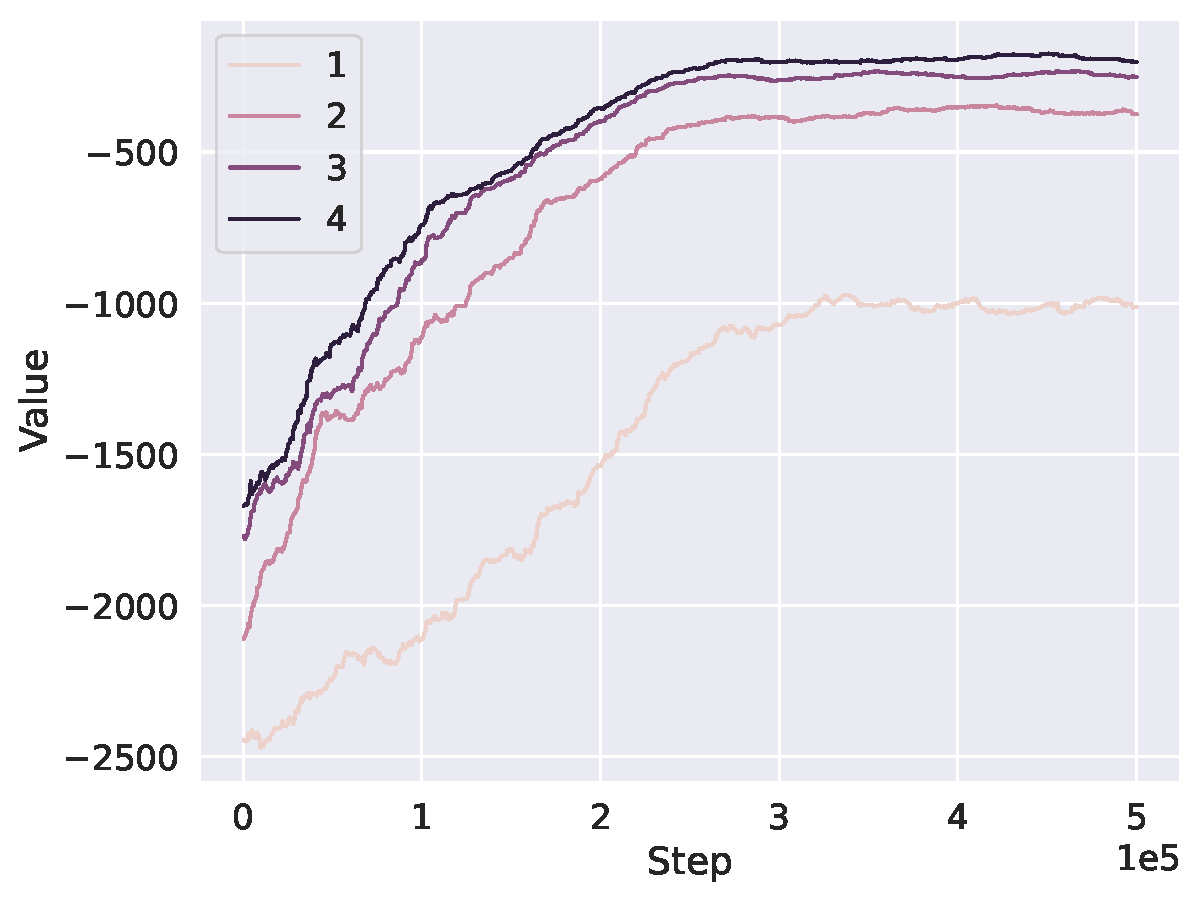
\includegraphics[width=0.9\textwidth]{../single-intersection/comparison.pdf}
  \caption{For the DQN, we use a fixed horizon of $h = 10$. The smoothed return
    obtained by a \textbf{single run} of the DQN algorithm is shown for each
    scenario.}
  \label{fig:dqn-learning-rates}
\end{figure}

% \bibliography{references}
% \bibliographystyle{ieeetr}

\end{document}
